%%%%%%%%%%%%%%%%%%%%%%%%%%%%%%%%%%%%%%%%%%%%%%%%%%%%%%%%%%%%%%%%%%%%%%
%%  Copyright by Wenliang Du.                                       %%
%%  This work is licensed under the Creative Commons                %%
%%  Attribution-NonCommercial-ShareAlike 4.0 International License. %%
%%  To view a copy of this license, visit                           %%
%%  http://creativecommons.org/licenses/by-nc-sa/4.0/.              %%
%%%%%%%%%%%%%%%%%%%%%%%%%%%%%%%%%%%%%%%%%%%%%%%%%%%%%%%%%%%%%%%%%%%%%%

\newcommand{\devtoolFigs}{../Web_Common/Figs}


% -------------------------------------------
% SUBSECTION
% ------------------------------------------- 
\subsection{Usando \texttt{"HTTP Header Live"} para inspeccionar Headers HTTP}
\label{web:sec:httpheaderlive}

La versión de Firefox 60 de nuestra Máquina Virtual de Ubuntu 16.04 no soporta el plugin \texttt{LiveHTTPHeader}, que fue usado en nuestra Máquina Virtual de Ubuntu 12.04.
Dada esta situación, se usará \texttt{"HTTP Header Live"} como reemplazo.
Las instrucciones de como habilitar y usar este plugin se muestran en la figura Figure~\ref{web:fig:httpheader} solamente haga click en el ícono mosotrado en el marcador \ding{192}; aparecerá una barra lateral en la izquierda, asegúrese que \texttt{HTTP Header Live} este seleccionada en la posición mostrada en el marcador \ding{193}. Luego haga click en cualquier link dentro de la página, todas los Requests HTTP serán capturados y mostrados dentro de la barra lateral mostrada en el marcador  \ding{194}.
Si hace click en cualquiera Request HTTP, se abrirá un pop-up que mostrará el Request HTTP seleccionado. Desafortunadamente hay un bug en este plugin (que aún se encuentra en desarrollo); no se mostrará nada dentro de este pop-up al menos que ud. cambie el tamaño del pop-up (Al parecer el evento de re-drawing se ejecuta automáticamente cuando se abre el pop-up, pero cambiando su tamaño ocasiona que este evento sea disparado y en consecuencia se renderize el contenido en pantalla)


\begin{figure}[htb]
\begin{center}
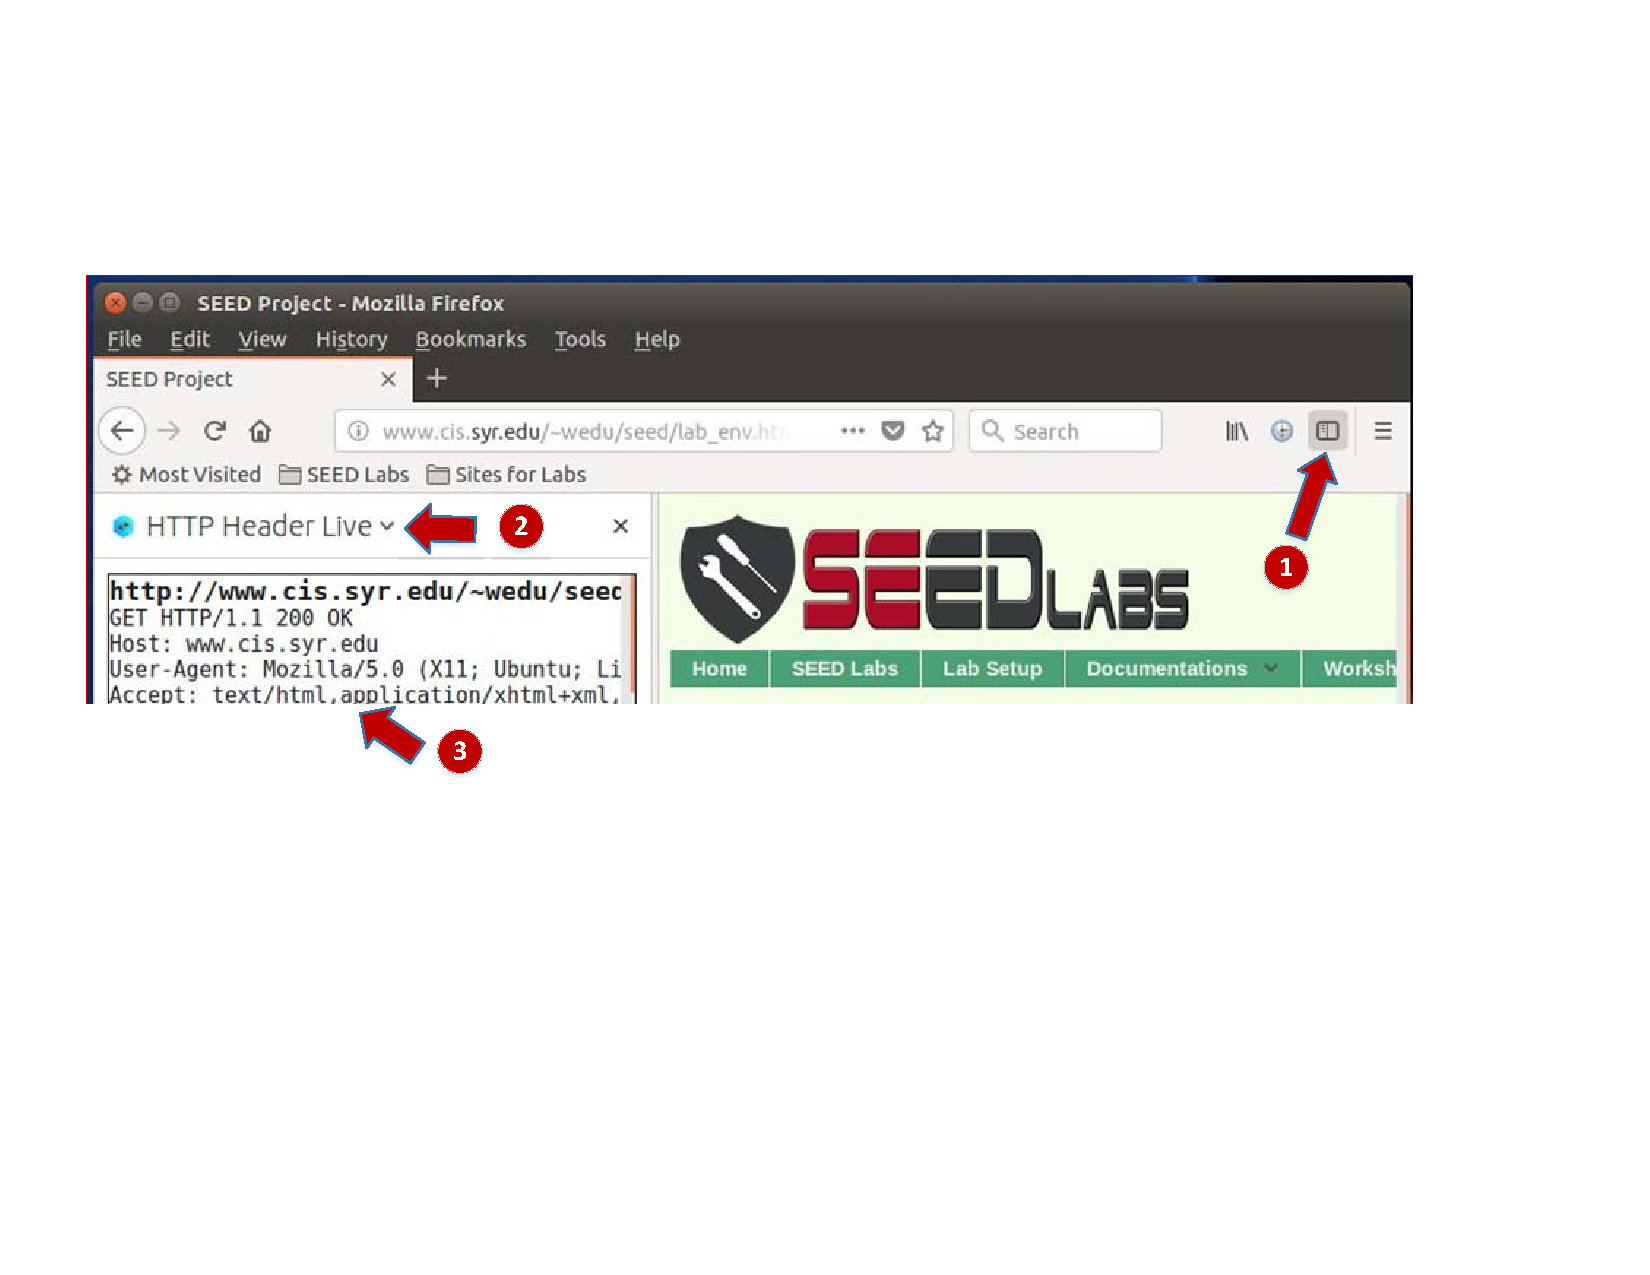
\includegraphics[width=0.85\textwidth]{\devtoolFigs/HTTPHeaderLive.pdf}
\end{center}
\caption{Hablitando el plugin HTTP Header Live}
\label{web:fig:httpheader}
\end{figure}




% -------------------------------------------
% SUBSECTION
% ------------------------------------------- 
\subsection{Usando Web Developer Tool para inspeccionar Headers HTTP}
\label{web:sec:web_dev_tools}

Existe otra herramienta provista por Firefox que puede ser muy útil para inspeccionoar Encabezados HTTP.
Esta herramienta es la Web Developer Network Tool. En esta sección, vamos a cubrir algunas de las features más importantes de esta herramienta.
La Web Developer Network Tool puede ser habilitada siguiendo estos pasos:

\begin{lstlisting}
Click Firefox's top right menu --> Web Developer --> Network
 or 
Click the "Tools" menu --> Web Developer --> Network 
\end{lstlisting}

Usaremos la página de login de Elgg como ejemplo.
La Figure~\ref{fig:webdevtools_01_request} muestra el Request HTTP POST que se envía al momento del login dentro de la Network Tool.

\begin{figure}[htb]
\begin{center}
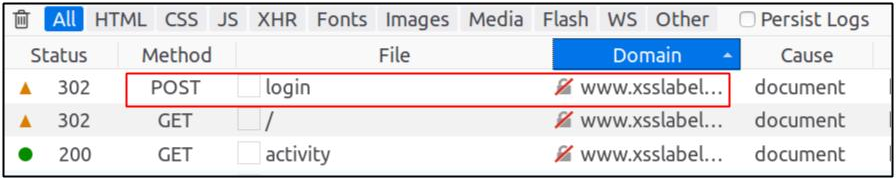
\includegraphics[width=0.8\textwidth]{\devtoolFigs/webdevtools_01_request.png}
\end{center}
\caption{Request HTTP en la Web Developer Network Tool}
\label{fig:webdevtools_01_request}
\end{figure}

Para más detalles del Request, podemos hacer click en un Request HTTP específico y se abrirán dos paneles con información detallada del mismo. (Ver Figure~\ \ref{fig:webdevtools_02_two_panes})

\begin{figure}[htb]
\begin{center}
	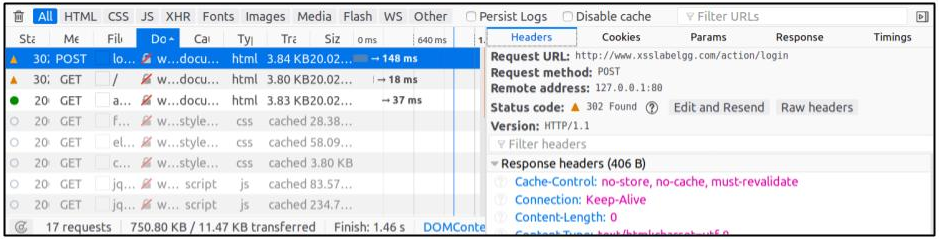
\includegraphics[width=0.95\textwidth]{\devtoolFigs/webdevtools_02_two_panes.png}
\end{center}
\caption{Request HTTP y Detalles del Request}
\label{fig:webdevtools_02_two_panes}
\end{figure}


Los detalles del Request seleccionado serán mostrados en el panel de la derecha.
La Figure~\ref{fig:webdevtools_03_post_headers} muestra los detalles del Request de Login en el Tab de 
\texttt{Headers} (Estos detalles incluyen el método del Request, la URL y la Cookie). En el panel derecho se pueden observar los Headers de la respuesta como también los del request.
Para chequear los parámetros involucrados en un request HTTP, podemos usar el tab \texttt{Params}. La Figure~\ref{fig:webdevtools_03_post_params} nos muestra los parámetros enviados en el request del login que se envía a Elgg, estos incluyen el \texttt{username} y el \texttt{password}. Esta herramienta puede ser usada para inspeccionar tanto Request HTTP GET como POST.

\begin{figure}[htb]
 \centering
 \subfigure[HTTP Request Headers]{
        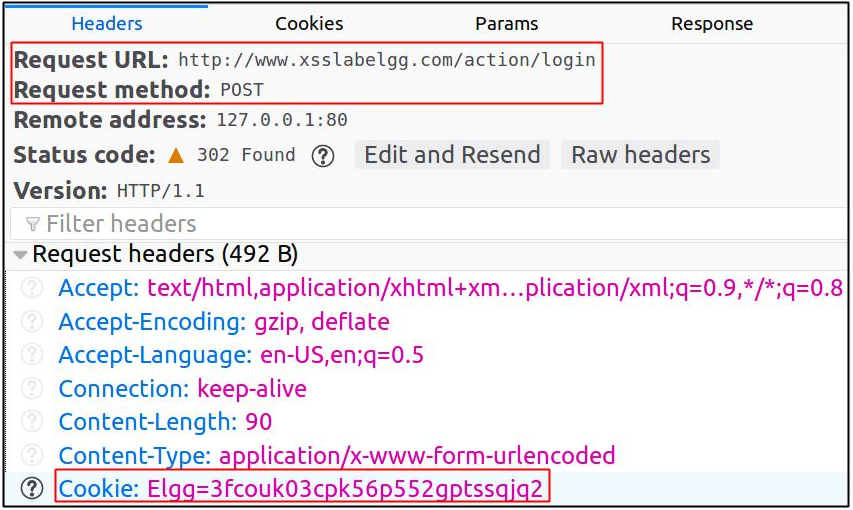
\includegraphics[width=0.6\textwidth]{\devtoolFigs/webdevtools_03-1.png}
        \label{fig:webdevtools_03_post_headers}
 }
 \subfigure[HTTP Request Parámetros]{
        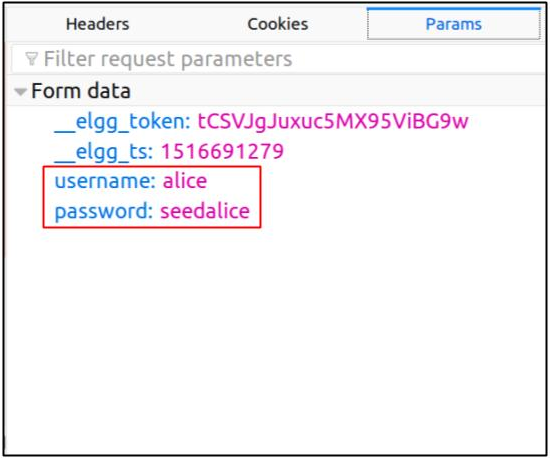
\includegraphics[width=0.35\textwidth]{\devtoolFigs/webdevtools_03-2.png}
        \label{fig:webdevtools_03_post_params}
 }
 \caption{HTTP Headers y Parámetros}
\end{figure}


\paragraph{Font Size.} El font size usado por defecto en la Web Developer Tool puede ser algo pequeño, para incrementar el tamaño de la fuente se debe hacer click en cualquier lugar de la ventana de la Network Tool y presionar en simultáneo las teclas \texttt{Ctrl} y \texttt{+} 



% -------------------------------------------
% SUBSECTION
% -------------------------------------------
\subsection{Debugueando JavaScript}
\label{web:sec:jsdebugging}

En muchas ocasiones vamos a necesitar debuguear nuestro código JavaScript. La developer tool de Firefox puede ayudarnos en esta tarea. Esta herramienta tiene la posibilidad de indicarnos el punto exacto en el código donde se produjo el error. A continuación se indica como habilitar el debugging en la Web Developer Tool:

\begin{lstlisting}
 Click the "Tools" menu --> Web Developer --> Web Console
 or use the Shift+Ctrl+K shortcut.
\end{lstlisting}

Una vez situados en la consola, se debe clickear en el tab {\tt JS}. Luego haga click en la flecha que apunta hacia abajo y asegúrese que al costado de {\tt Error} haya una tilde. Si también le interesa activar los mensajes de Warning en la coonsola seleccione {\tt Warnings}. Vea la Figure~\ref{devtool:fig:errocheckmark}.

\begin{figure}[htb]
\begin{center}
  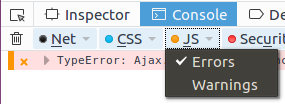
\includegraphics[width=0.4\textwidth]{\devtoolFigs/errorCheckMark.png}
\end{center}
\caption{Debugueando Código JavaScript (1)}
\label{devtool:fig:errocheckmark}
\end{figure}
 
Si hay errores en el código, se le mostrará un mensaje de error en la consola. Este mensaje indicará el número des línea que causó este error y estará ubicado en el extremo derecho del mensaje. Para ir al lugar exacto donde el código falló, deberá hacer click en el número de línea que es mostrado en el mensaje de error.
Vea la Figure~\ref{devtool:fig:console}.


\begin{figure}[htb]
\begin{center}
  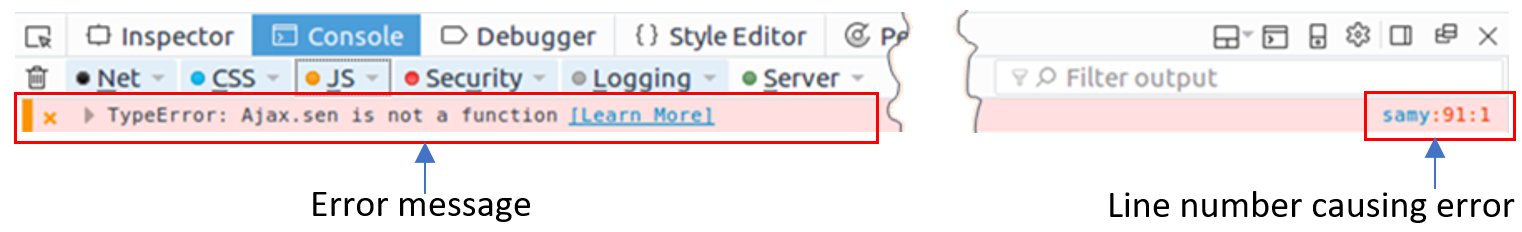
\includegraphics[width=1.0\textwidth]{\devtoolFigs/consoleError2.png}
\end{center}
\caption{Debugueando Código JavaScript (2)}
\label{devtool:fig:console}
\end{figure}
 




 
